%%%%%%%%%%%%%%%%%%%%%%%%%%%%%%%%%%%%%%%%%%%%%%%%%%%%%%%%%%%%%%%%%%%%%%%%%%%%%%%
\section{Test Cases}
\label{sec:Test Cases}
%%%%%%%%%%%%%%%%%%%%%%%%%%%%%%%%%%%%%%%%%%%%%%%%%%%%%%%%%%%%%%%%%%%%%%%%%%%%%%%

This paper models two test cases derived from the Benchmark for Evaluation And Validation of Reactor Simulations (BEAVRS) PWR model~\citep{horelik2013beavrs}. Each test case includes heterogeneous features -- and corresponding spatial self-shielding effects -- in order to understand their implications for accurate pin-wise MGXS generation. The impact of fuel enrichment, CRGTs, BPs, inter-assembly currents and water reflectors is considered. The geometric and material specifications for the two test cases are summarized in~\autoref{subsec:benchmarks}. The reference results computed with OpenMC for each of the test cases are discussed in~\autoref{subsec:metrics}.

-need to describe both pinwise fissoin rates and U-238 capture rates
  -latter papers can cite this one as reason to only analyze capture rates?


%%%%%%%%%%%%%%%%%%%%%%%%%%%%%%%%%%%%%%%%%%%%%%%%%%%%%%%%%%%%%%%%%%%%%%%%%%%%%%%
\subsection{Benchmark Configurations}
\label{subsec:benchmarks}

\begin{figure}[h!]
\centering
\begin{subfigure}{0.45\textwidth}
  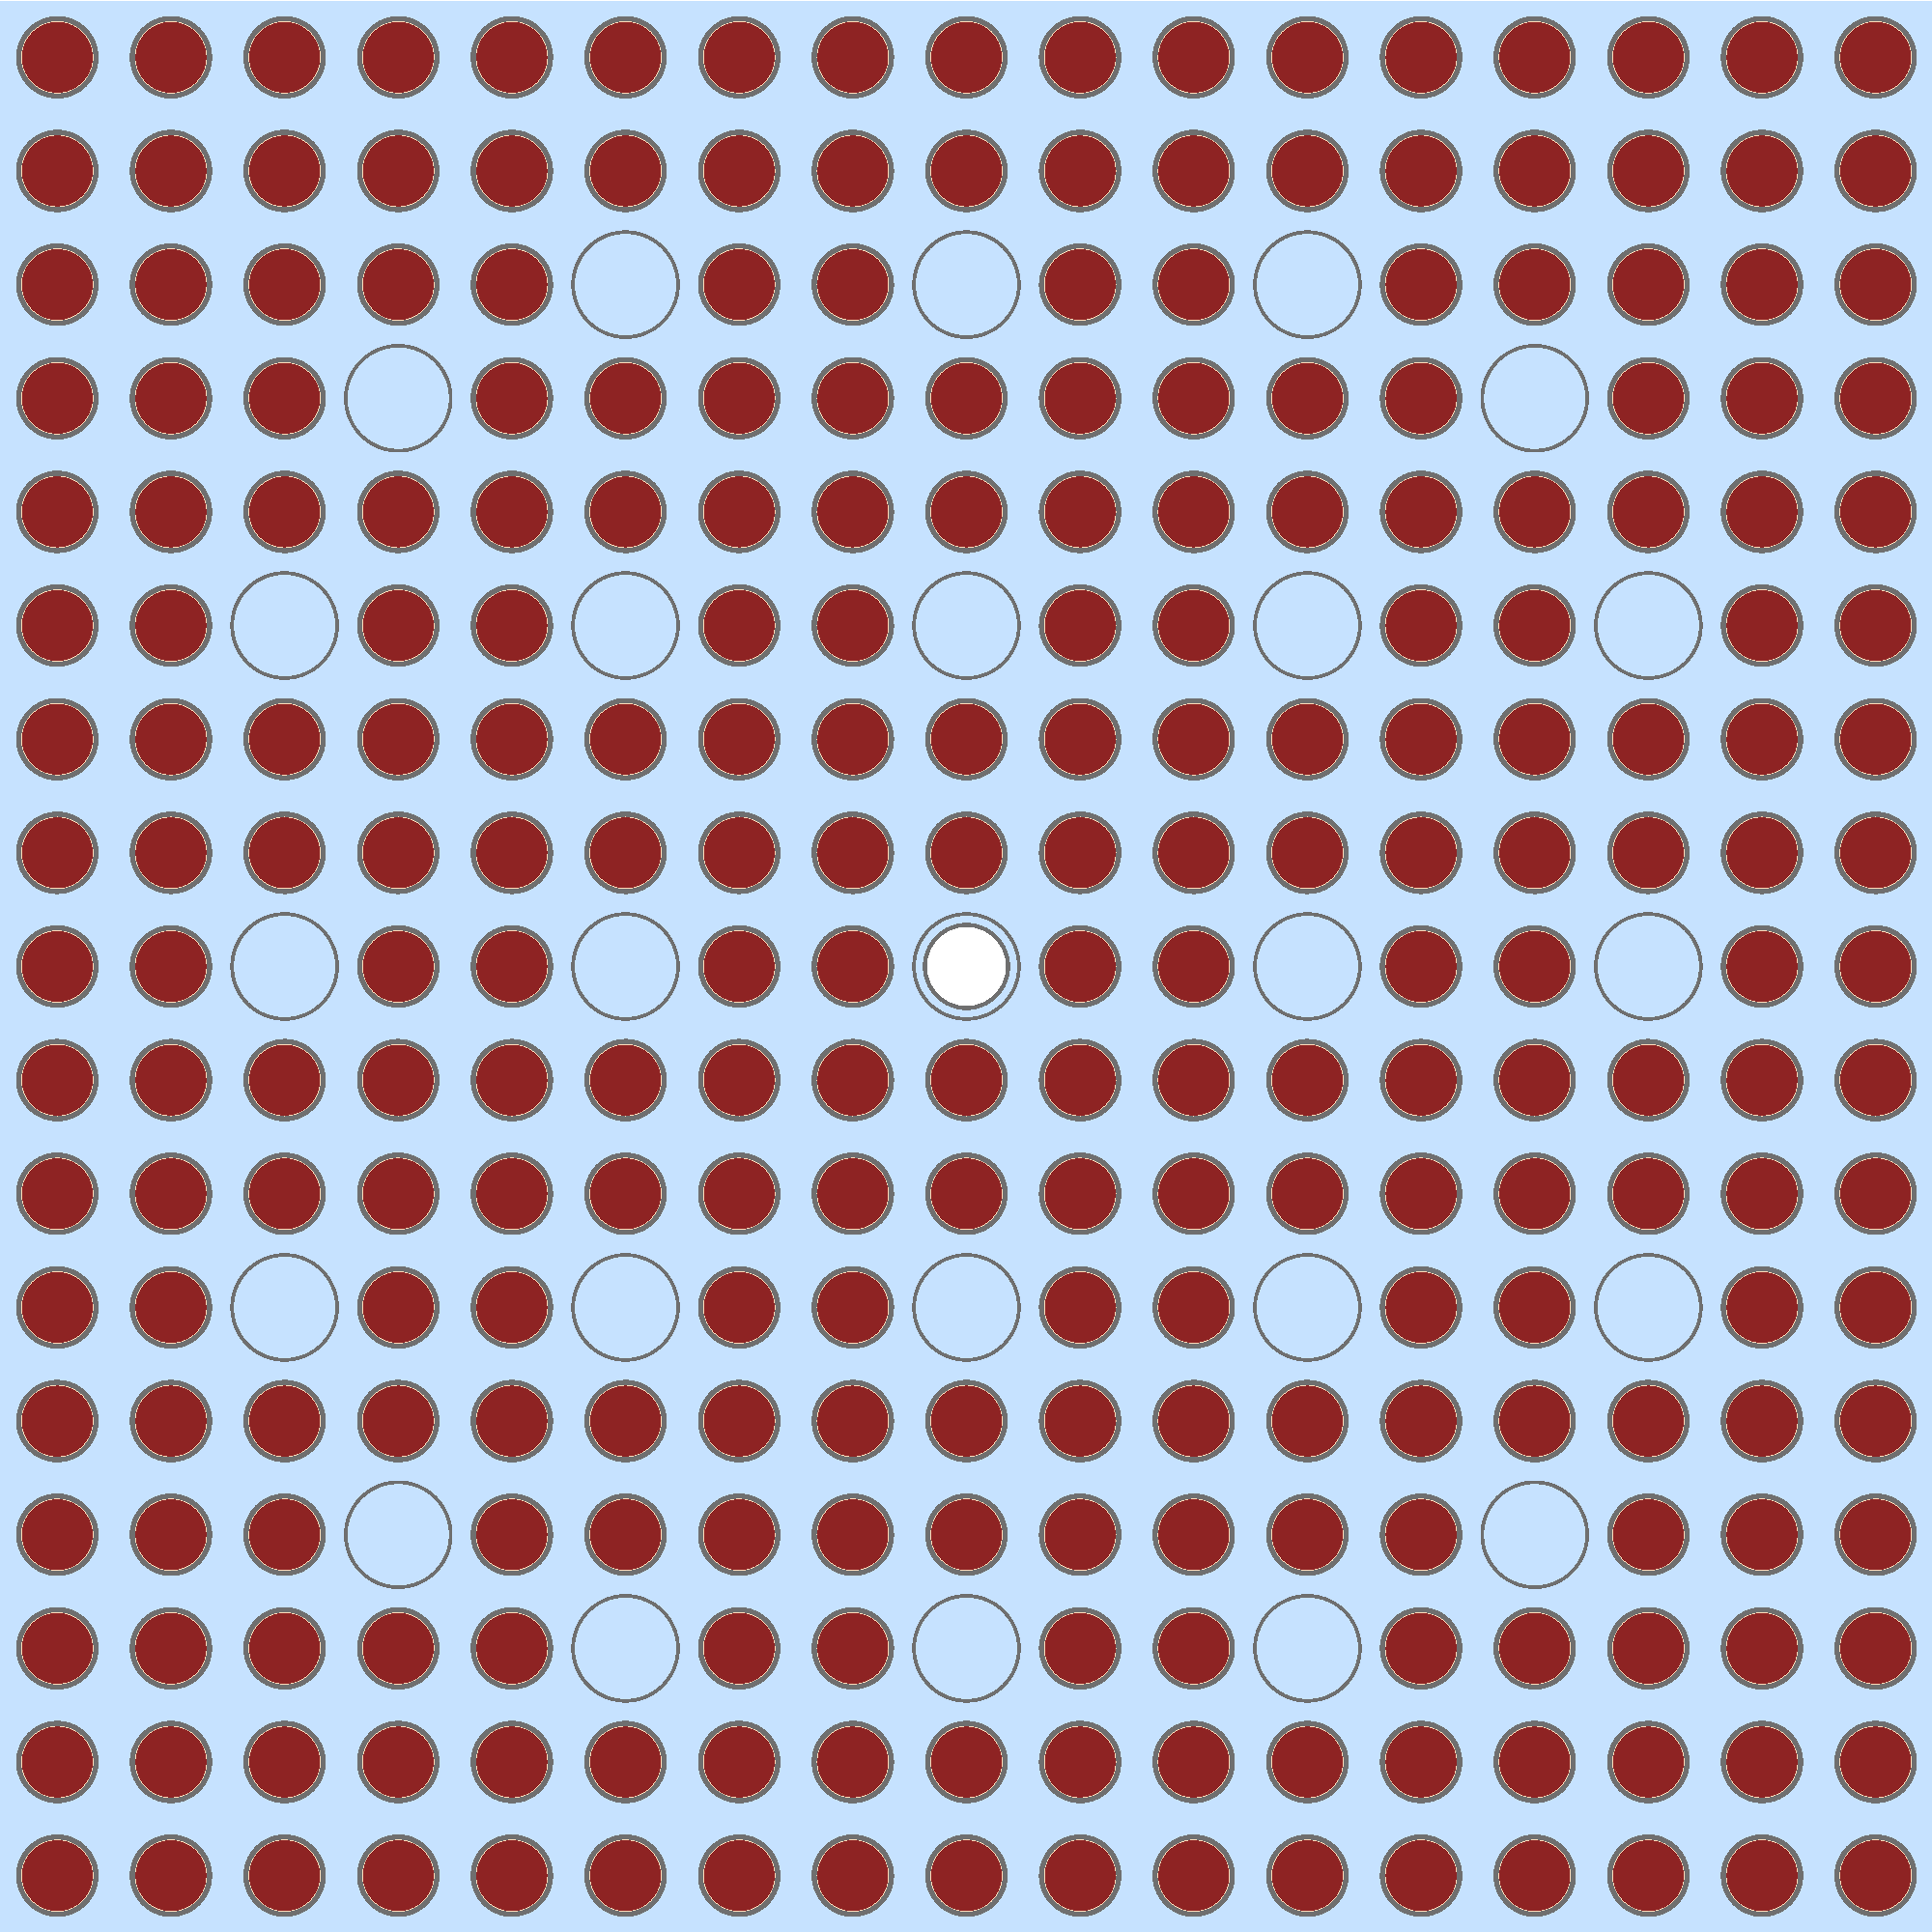
\includegraphics[width=\linewidth]{figures/assembly/geometry}
  \caption{}
  \label{fig:benchmarks-assm}
\end{subfigure}
\begin{subfigure}{0.45\textwidth}
  \centering
  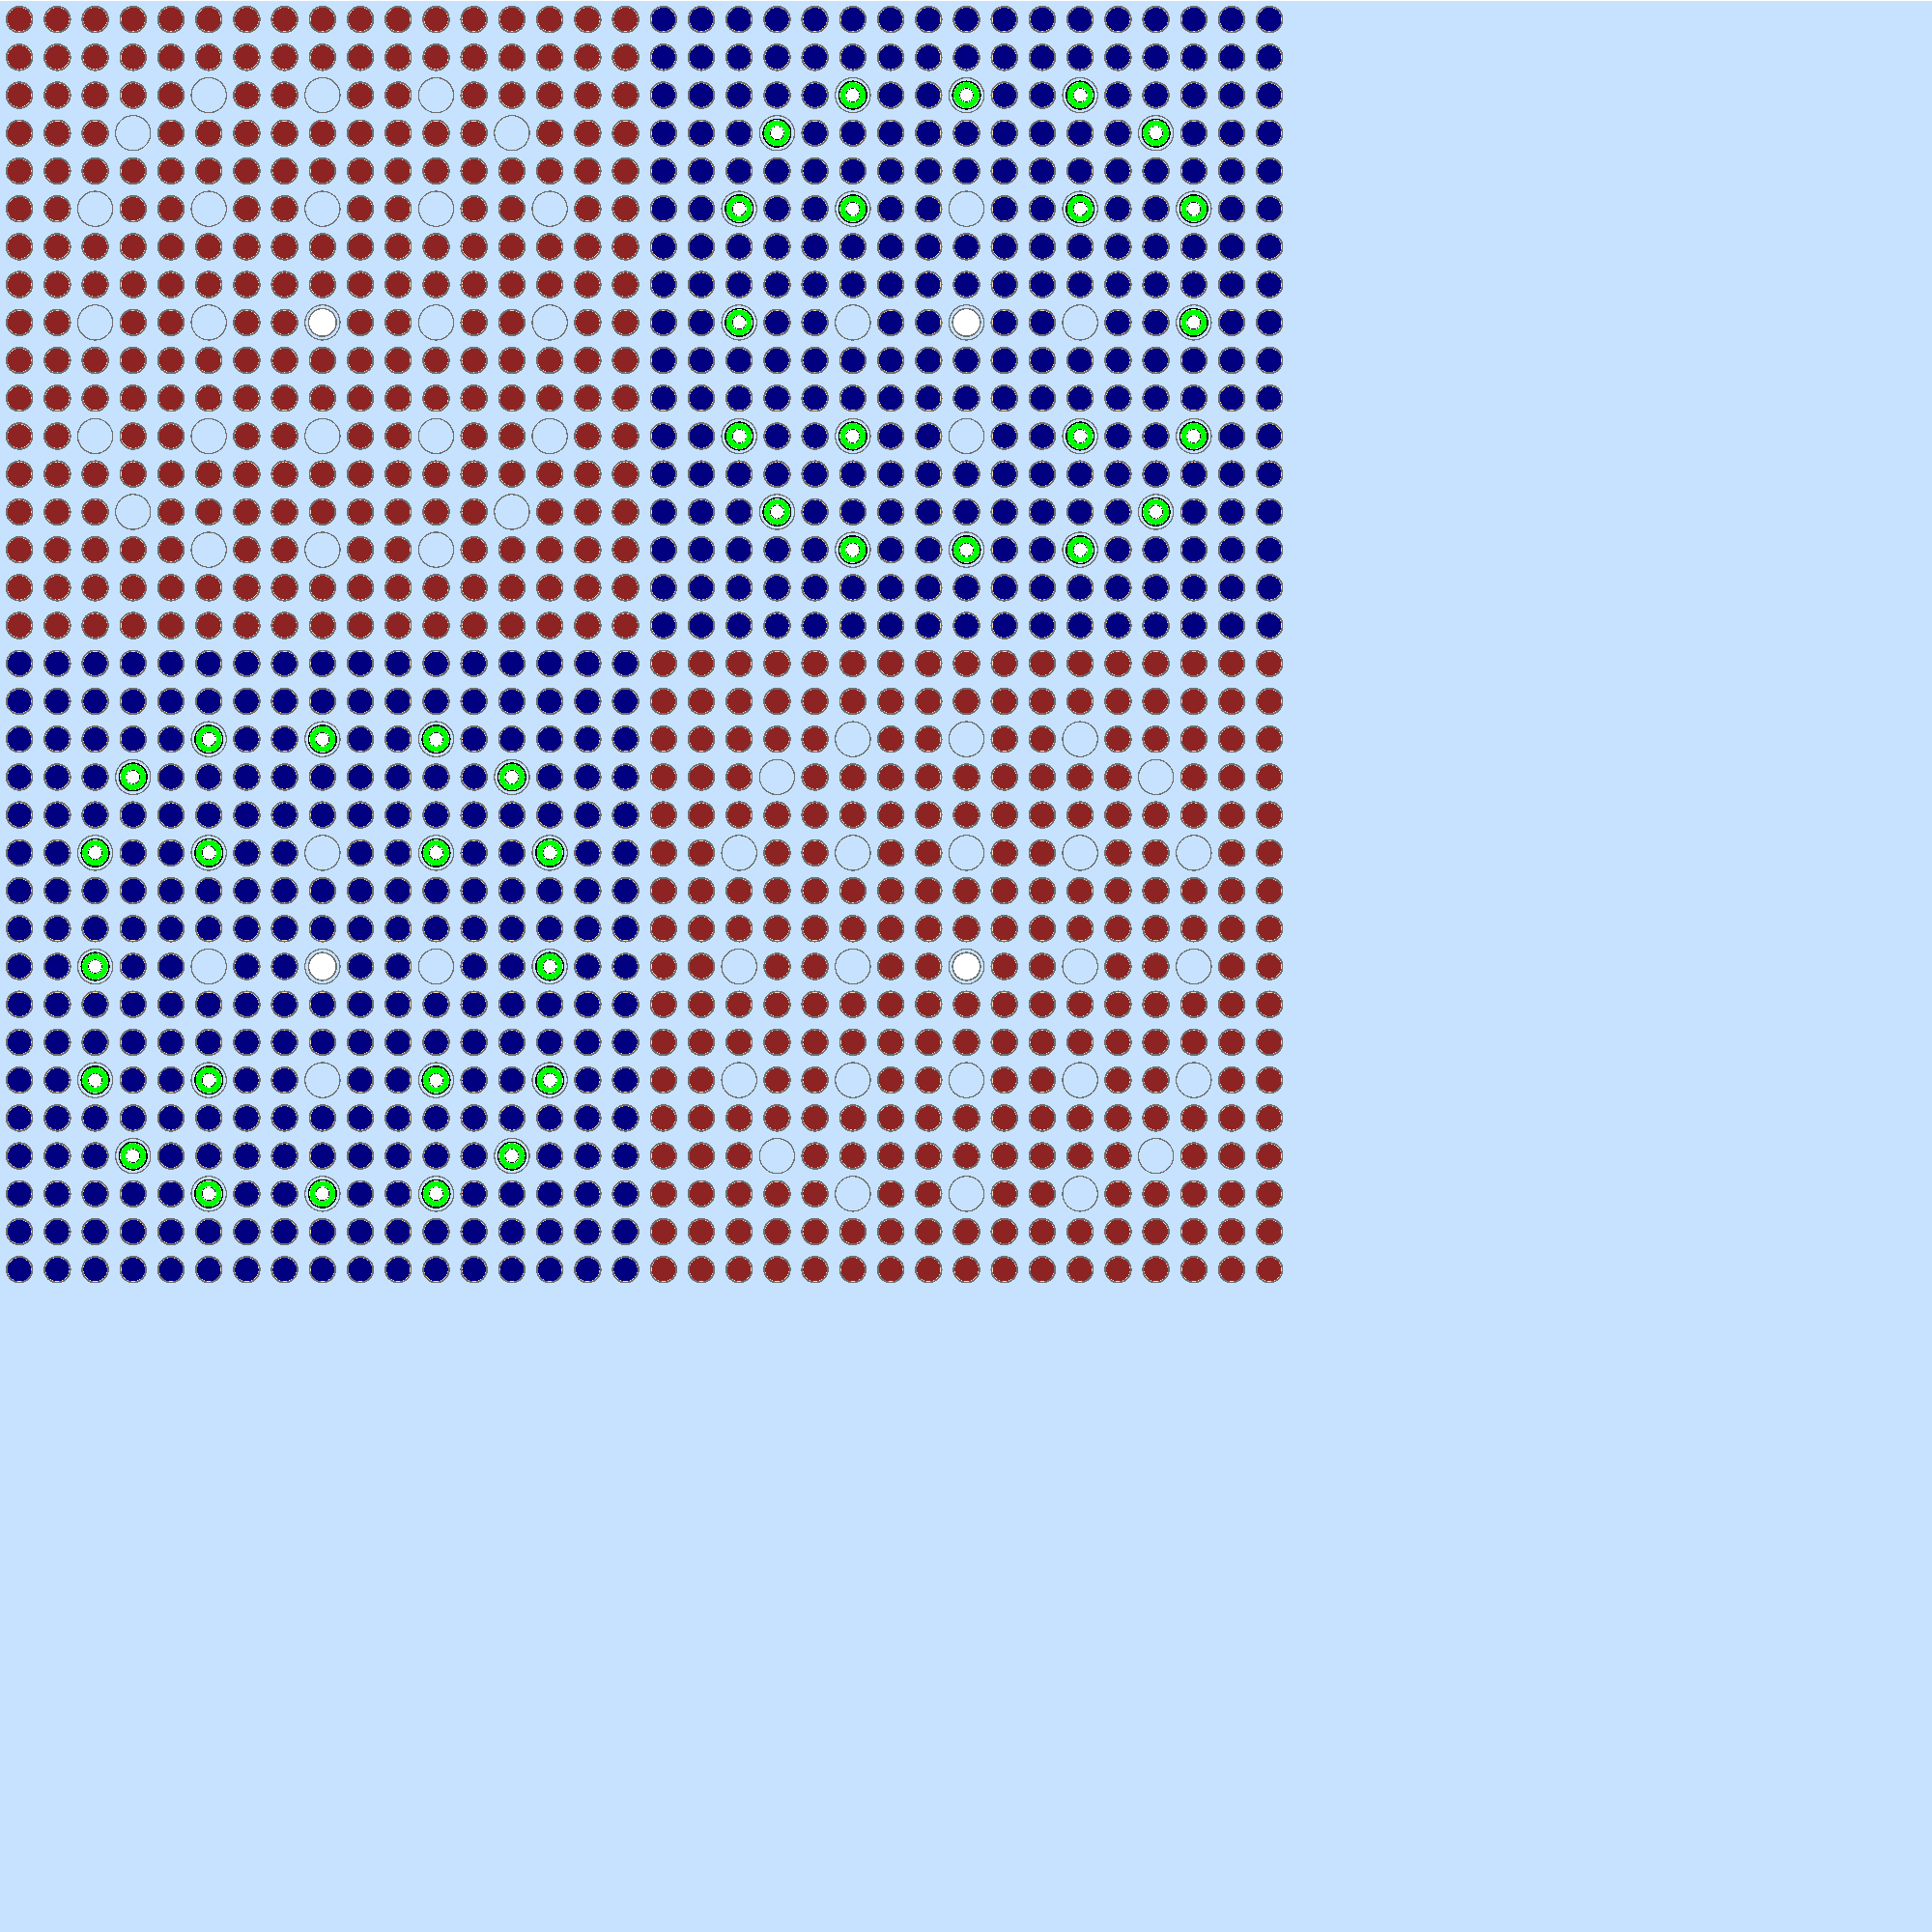
\includegraphics[width=\linewidth]{figures/reflector/geometry}
  \caption{}
  \label{fig:benchmarks-reflector}
\end{subfigure}
\caption{A (a) fuel assembly and (b) 2$\times$2 assembly colorset with reflector.}
\label{fig:benchmarks}
\end{figure}


%%%%%%%%%%%%%%%%%%%%%%%%%%%%%%%%%%%%%%%%%%%%%%%%%%%%%%%%%%%%%%%%%%%%%%%%%%%%%%%
\subsection{Single Fuel Assembly}
\label{subsubsec:benchmarks-assm}

%%%%%%%%%%%%%%%%%%%%%%%%%%%%%%%%%%%%%%%%%%%%%%%%%%%%%%%%%%%%%%%%%%%%%%%%%%%%%%%
\subsection{Reflected Assembly Colorset}
\label{subsubsec:benchmarks-2x2}



%%%%%%%%%%%%%%%%%%%%%%%%%%%%%%%%%%%%%%%%%%%%%%%%%%%%%%%%%%%%%%%%%%%%%%%%%%%%%%%
\subsection{Verification Metrics}
\label{subsec:metrics}

A series of OpenMC simulations were used to calculate reference eigenvalues, pin-wise fission rates, and pin-wise U-238 capture rates for both benchmarks. The ENDF/B-VII.1 continuous energy cross section libraries evaluated at 600K provided by the MCNP code~\citep{mcnpx2003manual} were used by OpenMC for all simulations. The reference solutions were computed with 100 inactive and 900 active batches of 10$^7$ particle histories per batch.

It should be noted that isotropic in lab scattering was employed for all reference calculations with OpenMC's ``iso-in-lab'' feature\footnote{The OpenMC ``iso-in-lab'' feature samples the outgoing neutron energy from the scattering laws prescribed by the continuous energy cross section library, but the outgoing neutron direction of motion is sampled from an isotropic in lab distribution.}. Although isotropic in lab scattering is a poor approximation for LWRs, it eliminated scattering source anisotropy as one possible cause of approximation error between OpenMC and OpenMOC in order to isolate approximation errors resulting from spatially self-shielded MGXS.

The reference eigenvalues are listed in~\autoref{tab:keff-reference}. The OpenMC ``combined'' eigenvalue estimator is reported along with the associated 1-sigma uncertainty of one pcm for both test cases.

\begin{table}[h!]
  \centering
  \caption{Reference OpenMC eigenvalues for each test case.}
  \label{tab:keff-reference} 
  \begin{tabular}{c c}
  \toprule
  {\bf Assembly} &
  {\bf Colorset} \\
  \midrule
  0.99326 $\pm$ 0.00001 & 0.94574 $\pm$ 0.00001 \\
  \bottomrule
\end{tabular}
\end{table}

The reference energy-integrated fission and U-238 capture rate spatial distributions were computed using rectilinear, pin-wise tally meshes in OpenMC and are shown in~\autoref{fig:fiss-capt-rates}. The reaction rates were volume-integrated across each fuel pin. The fission rates include fission from only U-235 and U-238 for the fresh PWR UO$_2$ fuel. The reaction rates were normalized to the mean of all non-zero reaction rates in each benchmark. The reaction rates in the instrument tubes, CRGTs and BPs are all zero and are illustrated in white. The 1-sigma uncertainties are less than 0.08\% in each pin for each benchmark.

\begin{figure*}[h!]
\centering
\begin{subfigure}{0.45\textwidth}
  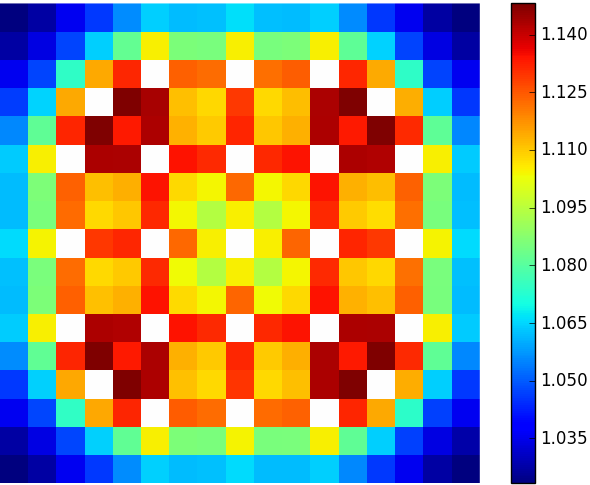
\includegraphics[width=\linewidth]{figures/assembly/fission-rates}
  \caption{}
  \label{fig:fiss-assm}
\end{subfigure}%
\begin{subfigure}{0.45\textwidth}
  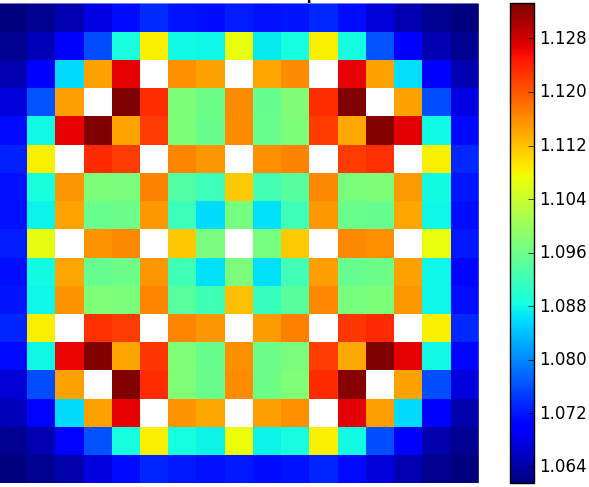
\includegraphics[width=\linewidth]{figures/assembly/capture-rates}
  \caption{}
  \label{fig:capt-assm}
\end{subfigure}
\begin{subfigure}{0.45\textwidth}
  \centering
  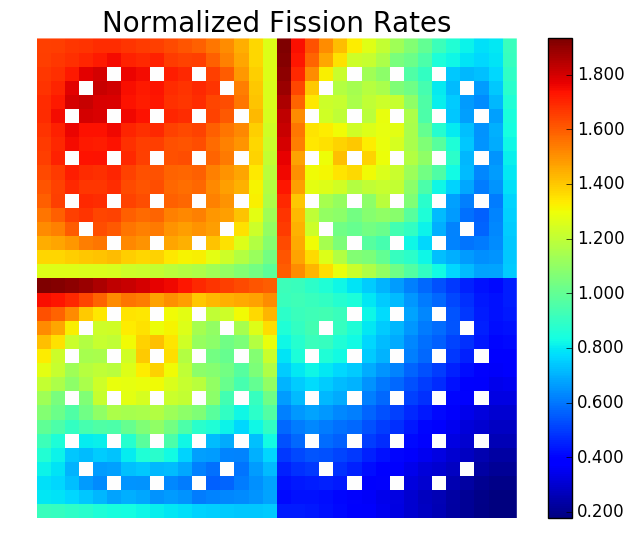
\includegraphics[width=\linewidth]{figures/reflector/fission-rates}
  \caption{}
  \label{fig:fiss-reflector}
\end{subfigure}%
\begin{subfigure}{0.45\textwidth}
  \centering
  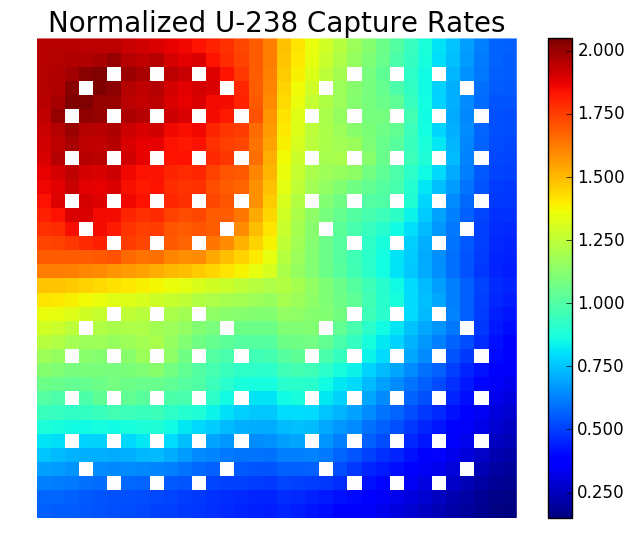
\includegraphics[width=\linewidth]{figures/reflector/capture-rates}
  \caption{}
  \label{fig:capt-reflector}
\end{subfigure}
\caption{Fission and U-238 capture rates for the (a) -- (b) assembly and (c) -- (d) colorset.}
\label{fig:fiss-capt-rates}
\end{figure*}

As illustrated in the figures, the reaction rate rate distributions are strongly dependent on the spatially heterogeneous features in each benchmark. For example, the CRGTs provide additional moderation and increase the fision and U-238 capture rates in nearby fuel pins. The inclusion of BPs reduces the neutron population and therefore the reaction rates for the surrounding fuel pins. The presence of a reflector with a mixture of vacuum and reflective BCs induces a tilt in the reaction rates across the assemblies in the colorset.

Although spatial heterogeneities generally have similar effects on both fission and U-238 capture rates, there are a few important differences to note. The U-238 capture rates in the assemblies are more sensitive than the fission rates to the spatial self-shielding induced by moderation in CRGTs. In addition, the capture rates in the colorset are more smoothly varying at the inter-assembly and assembly-reflector interfacea than the fission rates.